%!TEX root = report.tex

\chapter{Travail Accompli}

\section{Introduction du chapitre}

Dans ce chapitre on procède à la présentation des cas utilisateur de
notre système ainsi que l'identification des acteurs impliqués dans ces
cas. Puis on décortique l’implémentation que nous proposons en citant
éventuellement nos motifs et intentions.

\section{Vue Générale}
\subsubsection{Identification des acteurs}

Notre système interagit essentiellement avec trois acteurs différents:

\begin{description}
\item[Le médecin] C'est l'acteur principal de notre système.

\item[Le service web] Source des données à acheminer vers le médecin.

\item[Système d'exploitation] Communique à notre système les
informations recueillies des divers composants qui nous intéressent
(localisation GPS/Network, état de la connectivité, état de la
batterie).

\end{description}

\subsection{Cas d'utilisations}

\begin{figure}
\center
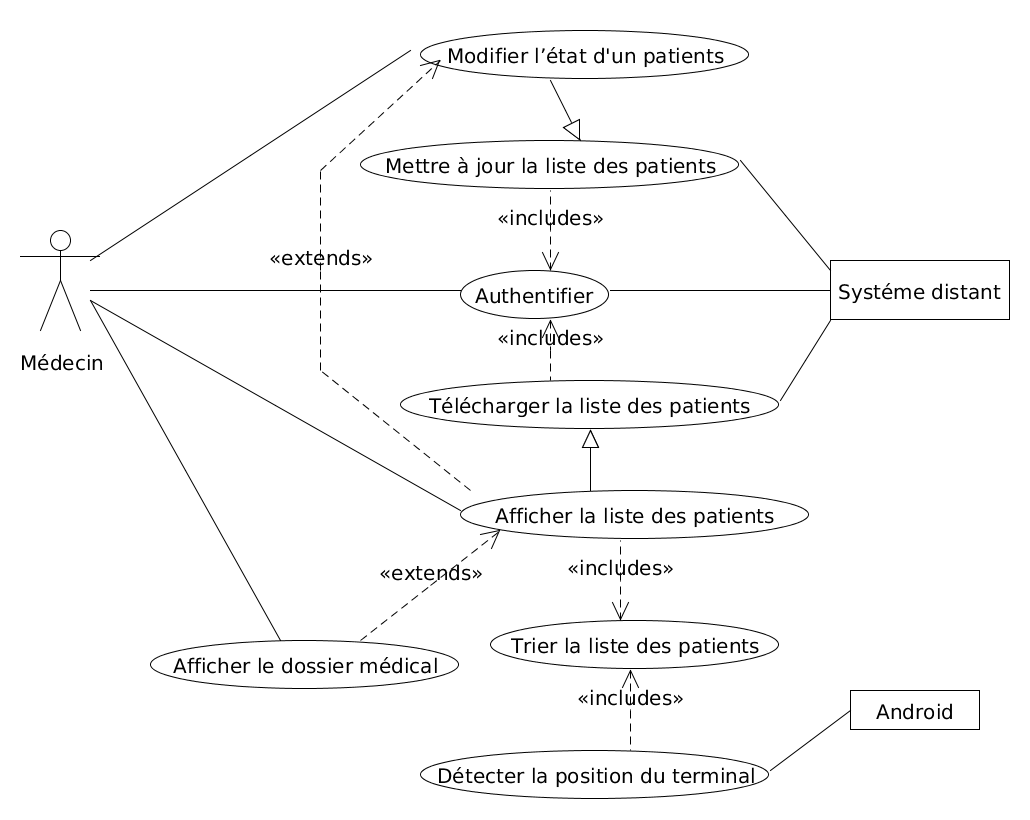
\includegraphics[width=0.8\textwidth]{diagrams/usecases}
\caption{Diagramme \gls{uml} des cas d'utilisation.}
\label{fig:usecase}
\end{figure}

\subsubsection{Cas: Authentifier}
\subsubsection{Cas: Notifier la proximité d'un patient}
\subsubsection{Cas: Détecter la position du terminal}
\subsubsection{Cas: Afficher la liste des patients}
\subsubsection{Cas: Télécharger la liste des patients}
\subsubsection{Cas: Modifier la liste des patients}
\subsubsection{Cas: Mettre à jour la liste des patients}

\subsection{Environnement de développement}%TODO
Plusieurs outils on était mise à contribution pour développer l'application, tant que sur le plan logiciel que matériel.

\subsubsection{Environnement Logiciel}
Voici une liste des outils logiciels utilisés pendant le développement de l'application.

\begin{description}

\item [Ubuntu 12.04] Système d'exploitation.\footnotemark[1]

\item [OpenJDK 6] \gls{jdk} version 6.\footnotemark[2]

\item [Eclipse Juno] Environnement de Développement Intégrer dans sa version \en{Service Release 2}.\footnotemark[3]

\item [\gls{adt} (plugin Eclipce)] Intégration des outils de développement fournit dans l'\gls{sdk} \android{}.\footnotemark[4]

\item [ObjectAid (plugin Eclipce)] Génération des diagrammes de classes.\footnotemark[5]

\item [PlantUML (plugin Eclipce)] Génération des diagrammes de séquences.\footnotemark[6]

\item [Git] Gestionnaire des versions\footnotemark[7].

\item [EGit (plugin Eclipse)] Intégration du gestionnaire de version.\footnotemark[8]

\item [Evolus Pencil] Génération de prototypes et des sketchs\footnotemark[9]
\end{description}

\footnotetext[1]{http://www.ubuntu.com}
\footnotetext[2]{http://openjdk.java.net}
\footnotetext[3]{http://www.eclipse.org}
\footnotetext[4]{https://developer.android.com/tools/sdk/eclipse-adt.html}
\footnotetext[5]{http://www.objectaid.com/}
\footnotetext[6]{http://plantuml.sourceforge.net/}
\footnotetext[7]{ttp://git-csm.com}
\footnotetext[8]{http://www.eclipse.org/egit/}
\footnotetext[9]{http://pencil.evolus.vn/}

\subsubsection{Environnement Matériel}
Le développement de l'application est fait avec une tablette Asus Nexus 7 (mise à jour à \android{} 4.2.2 \en{Jelly Bean}).

\section{Architecture Générale}

L'architecture globale de l'application (figure \ref{fig:cls_global})
est calquée sur Le patron "Vue Passive" (Passive View Pattern). Le patron
\en{Passive View} (fig \ref{fig:passive_view}) est une variation des
patrons \gls{mvc} et \gls{mvp}, de ce qui ce passe dans ces patrons.

L'interface utilisateur est divisée entre une vu qui s'occupe de
l'affichage des données et un contrôleur qui répond aux interactions de
l'utilisateur. La différence majeur avec le \en{Passive View} est que la
vue est complètement passive et n'ai pas responsable de sa mise à jour
depuis le modèle. Dans ce cas toute la logique de la vue est dans le
contrôleur et aucune dépendance ni dans un sens au dans un autre entre
le vue et le modèle~\cite{fowler:passive_view}.

\begin{figure}[H]
\center
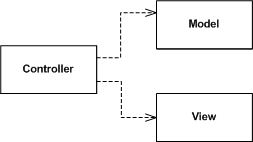
\includegraphics[width=0.6\textwidth]{passive_view}
\caption{Diagramme \gls{uml} du patron \en{Passive Viev}~\cite{fowler:passive_view}}
\label{fig:passive_view}
\end{figure}

Ce patron est idéal dans notre cas pour deux raisons majeures:

\begin{itemize} 

\item Dans notre projet la vu n'est pas la partie la plus importante
dans la mesure où l'objectif est d'intégrer un système développé
parallèlement, donc éventuellement avec une autre logique de
présentation. Déporter les interactions avec le modèle dans le
contrôleur permet d'intégrer d'autres implémentations d'affichage plus
facilement.

\item La nature même de cette procédure d’accès - à savoir l’aspect
abstrait, donc plus fragile - nous conduit à réduire les composants en
relations pour réduire la marge d'erreur possible et facilité les tests d’intégration.

\end{itemize}

\begin{figure}
\center
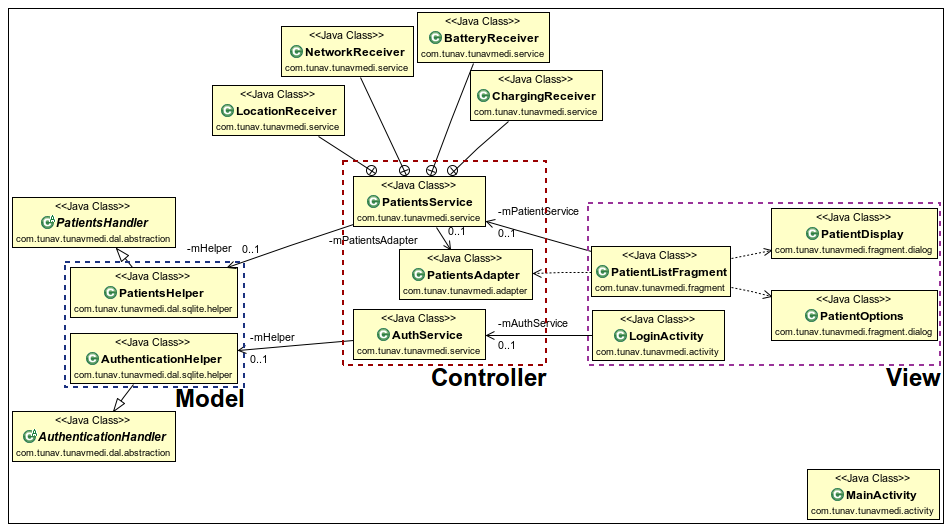
\includegraphics[angle=90, width=0.8\textwidth]{clsglobalhighlights}
\caption{Architecture générale de l'application.}
\label{fig:cls_global}
\end{figure}

Dans la suite de ce chapitre, on procède à l'explication détaillée de chaque composant de cette architecture.

\section{Le Modèle} 

Un des objectifs de ce projet étant de fournir une solution d’accès aux
données flexibles à fin de couvrir les besoins de chaque client de
manière individuelle. On a opté donc pour un modèle basé sur
l’implémentation de deux interfaces (figure \ref{fig:adl}):

\begin{itemize}
\item Interface d'authentification.
\item Interface d’accès à la liste des patients.
\end{itemize}

\begin{figure}
\center
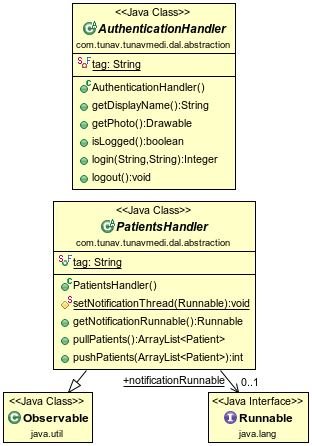
\includegraphics[totalheight=0.5\textheight]{diagrams/cls_adl}
\caption{Diagramme de classes des interfaces de la couche d’accès.}
\label{fig:adl}
\end{figure}

L'idée est simple: pour chaque client, une implémentation spécifique à son infrastructure sera développée soit par son propre effectif, soit par une des équipes de \textsc{Tunav}, ou dans le cas idéal par une alliance formé par des agents des deux camps qui garantie une collaboration plus poussée pour des résultats meilleurs.
Ces ensembles d'interfaces nous permettent de construire notre application.

\subsection{Implémentation de tests} 

Le package \dev{com.tunav.tunavmedi.dal.sqlite} contiens une
implémentation de la couche d’accès abstraite (figure
\ref{fig:adl_sqlite}) est réalisée dans le cadre de ce projet pour
pouvoir tester la solution. Cette implémentation est de caractère local
à l'application à travers les \gls{api} de la base de données
\dev{SQLite} qui fait parti de l'\gls{sdk} \android{}. En fait une
implémentation locale nous affranchie des problèmes qui peuvent se
produire dont la corrélation avec l'application est faible. Cette même
idée a influencé la mise en place même de cette implémentation qui à su
rester la plus simple possible en restant très proches des objets de
base de notre application.

\begin{figure}
\center
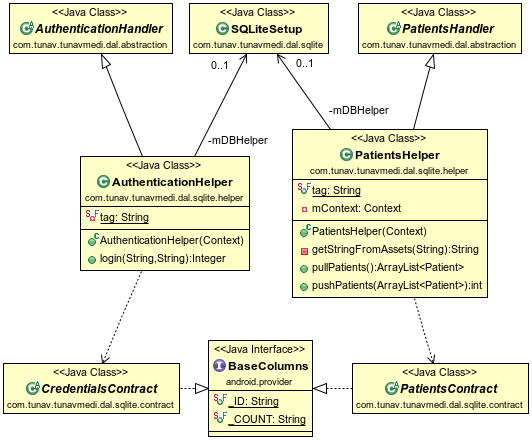
\includegraphics[angle=90, width=\textwidth]{diagrams/cls_adl_sqlite}
\caption{Diagramme de classe de l'implémentation de la couche d'accès de test à base de SQLite.}
\label{fig:adl_sqlite}
\end{figure}

Cette implémentation peut être subdivisée en trois éléments: Les \dev{Contrats}, les \dev{Helpers}, et la classe \dev{DBSetup}.

\paragraph{Les Contrats:}

Représente les contrats relative aux tables dans notre implémentation de
test. Chaque contrat implémente l'interface
\dev{android.provider.BaseColumns} et contient - entre autre - les
commandes SQL de création et de suppression de la dite table, des
éventuel index, et les commande d'insertion des données de test.

\paragraph{Les \en{Helpers}:} 

Ce sont les implémentations des classes abstraites qui définisse la
couche d’accès et présente les procédure d'extraction des données pré-
inséré dans nos table fictives en faisant appel à la classe
\dev{DBSetup} .

\paragraph[La classe \dev{DBSetup}:]{La classe \dev{DBSetup}:} 

Elle hérite de la classe \dev{SQLiteOpenHelper} et est destiner à
contrôler la création et l’accès à notre base de données de teste.

\subsection{Interface d'authentification}

\dev{com.tunav.tunavmedi.dal.abstraction.AuthenticationHandler} (figure
\ref{fig:cls_adl_auth}) est une classe abstraite comportant les méthodes
requise par notre application pour effectué les actions
d'authentification, de dé-authentification, de vérification
d'authenticité ainsi l'obtention des informations associées à l'utilisateur
authentifier.

Malgré la variété des techniques d'authentification utilisée dans le
domaine informatique, l'étape d'acquisition des identificateurs de
l'utilisateur représente un point de départ commun. On utilise ce
caractère dans l'interface d'authentification en demandant à nos clients
d'implémenter la méthode \dev{login()} qui prend en argument
l'identifiant et le mots de passe fourni par le médecin. Pour effectuer
l’opération inverse le client implémente la méthode \dev{logout()}
supposée annoncer au service distant la dé-authentification de
l'utilisateur du terminal. Pour verifier le l'état actuel de la relation
du terminal avec la base distante, on utilise le booléen retourné par
\dev{isLogged()}, utile dans les cas de déconnexion temporaire ou du
redémarrage de notre application. les méthodes \dev{getDisplayName()} et
\dev{getPhoto()} retournent respectivement le nom de l'utilisateur et sa
photo.

\begin{figure}[H]
\center
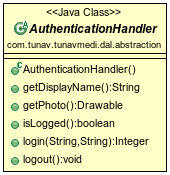
\includegraphics[scale=1]{diagrams/cls_adl_auth}
\caption{Diagramme de classe de l'interface d'authentification.}
\label{fig:cls_adl_auth}
\end{figure}

\subsection{Interface d’accès à la liste des patients}

\dev{com.tunav.tunavmedi.dal.abstraction.PatientsHandler} (figure
\ref{fig:cls_adl_patient}) est une classe abstraite comportant les méthodes
requise par notre application pour effectué les actions de mise à jour de la liste des patients dans le deux sens (terminal $\rightarrow$ service et terminal $\leftarrow$ service), elle contient aussi un objet de type \dev{Runnable} associé au mécanisme de notification.

\begin{figure}[H]
\center
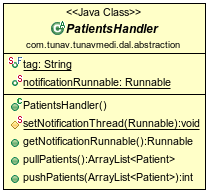
\includegraphics[scale=1]{diagrams/cls_adl_patient}
\caption{Diagramme de classe de l'interface d’accès à la liste des patients.}
\label{fig:cls_adl_patient}
\end{figure}

\subsubsection{Mécanisme de notification}

Le patron \textbf{Observateur} (\en{observer pattern}) (fig
\ref{fig:observer}) et un patron de conception couramment utilisé et qui
nous permet d'avoir une relation 1$\rightarrow$N entre divers objets. Le
patron observateur assume que l'objet qui contient les données est
séparé des l’objet qui les affiche et ces dites objets observe le
changement de ces données~\cite{jdp_observer}. Quant on implémente le
patron observateur, on réfère communément à l'objet contenant les
données par "Sujet"; et chacun des consommateurs des données par
"Observateur", Et chaque Observateurs implémente une interface préconçu
que le Sujet invoque quant les données changes~\cite{jdp_observer}.

\begin{figure}[H]
\center
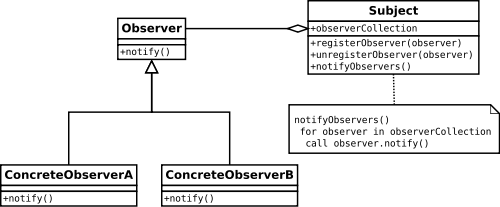
\includegraphics[width=0.8\textwidth]{Observer}
\caption{Diagramme UML du patron de conception Observateur~\cite{wiki:observer}}
\label{fig:observer}
\end{figure}

Dans le langage Java, ce patron est réalisé à travers la classe \dev{java.util.Observable} et l'interface \dev{Java.util.Observer}. Le Sujet hérite de la classe \dev{Observable} et les changements sont signalés par les méthodes \dev{setChanged()} et \dev{notifyObservers()} ou \dev{notifyObservers(Object message)}.


\section{Le Contrôleur}

\subsection{Localisation}

\subsection{Algorithme de Trie}

\subsection{Conscience de l'état du terminal}

\begin{table}[H]
\centering
\begin{tabular}{|c|c|c|}
\hline
&\textsf{Mises à jour} & \textsf{Localisation}\\
\hline
\textsf{Batterie Faible} & déactivé & déactivé\\
\hline
\textsf{Batterie en Charge} & activé & déactivé\\
\hline
\textsf{Pas de connectivité} & déactivé & activé\\
\hline
\end{tabular}
\end{table}

\subsubsection{Connectivité}

\begin{lstlisting}[language=xml, caption=Permission d’accès à l’état des interfaces réseaux.]

<uses-permission android:name="android.permission.ACCESS_NETWORK_STATE" />

\end{lstlisting}

\begin{lstlisting}[language=xml, caption=Enregistrement du  NetworkReceiver aux événements liée au status des interfaces réseaux.]

        <receiver
            android:name="com.tunav.tunavmedi.broadcastreceiver.NetworkReceiver"
            android:enabled="true" >
            <intent-filter>
                <action android:name="ConnectivityManager.CONNECTIVITY_ACTION" />
            </intent-filter>
        </receiver>

\end{lstlisting}

\subsubsection{Batterie}

\begin{lstlisting}[language=xml, caption=Enregistrement du BatteryReceiver aux événements liée à l’état de la batterie.]

        <receiver
            android:name="com.tunav.tunavmedi.broadcastreceiver.BatteryReceiver"
            android:enabled="true" >
            <intent-filter>
                <action android:name="android.intent.action.BATTERY_LOW" />
                <action android:name="android.intent.action.BATTERY_OK" />
            </intent-filter>
        </receiver>

\end{lstlisting}



\subsubsection{Mobilité}

\begin{lstlisting}[language=xml, caption=Enregistrement du ChargingReceiver aux événements liée au status de chargement.]

        <receiver
            android:name="com.tunav.tunavmedi.broadcastreceiver.ChargingReceiver"
            android:enabled="true" >
            <intent-filter>
                <action android:name="android.intent.action.ACTION_POWER_CONNECTED" />
                <action android:name="android.intent.action.ACTION_POWER_DISCONNECTED" />
            </intent-filter>
        </receiver>

\end{lstlisting}

\section{La Vue}
Le système d'exploitation \android{} rend facile le développement des applications qui tourne sur des appareils qui possèdes des formes et des tailles d’écran différents, une des améliorations

\section{Détecteur de bugs: Android Lint}

\begin{figure}[H]
\center
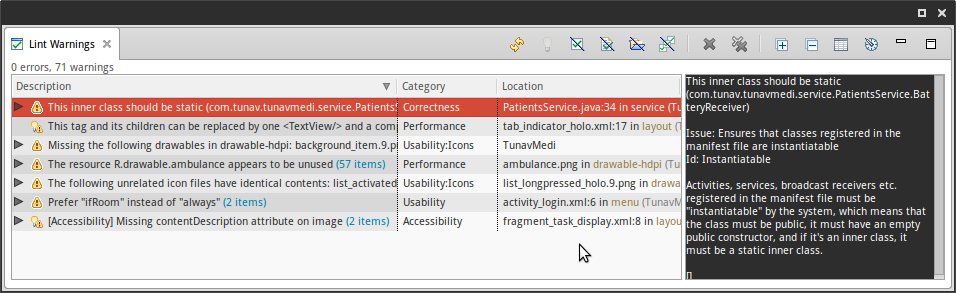
\includegraphics[width=0.9\textwidth]{lint}
\caption{Problèmes potentiels dans notre application détectés par Android Lint.}
\label{fig:lint}
\end{figure}

\android{} \en{Lint} (figure \ref{fig:lint}) est un outil introduit dans la version 16 de \gls{adt} qui scanne les code sources des projets \android{} afin d'y détecter des mal-fonctions potentiels.

Quelques exemples de types d'erreurs que cet outil permet de détecter sont:

\begin{itemize}

\item Translations manquantes ou inutilisés.

\item Les problèmes de performance dans les \dev{Layout}.

\item Ressources inutilisées

\item Tableau de taille inconsistante (dans le cas ou le tableau est défini dans des configurations différentes).

\item Problème d'accessibilités et d'internationalisation.

\item Problème d'icônes (Tailles manquantes, doubles, fausse résolution).

\item Problème d'usabilité .

\item Erreurs dans le \dev{Manifest}.

\end{itemize}

Dans Eclipse, \android{} Lint est disponible à travers le menu Window $\rightarrow$ Show View $\rightarrow$ Other... puis on sélectionne \en{Lint Warning} dans la fenêtre qui s'affiche (figure \ref{fig:lint_eclipse}).

\begin{figure}
\center
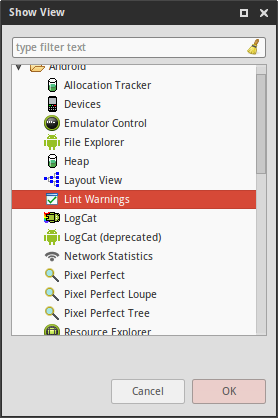
\includegraphics[width=0.4\textwidth]{lint_eclipse}
\caption{Accéder à Android Lint dans Eclipse}
\label{fig:lint_eclipse}
\end{figure}

\section{Conclusion du chapitre}